% CSE 713 — Artificial Intelligence
% Search Algorithms: Complete Model Answers (2020–2024)
% University of Chittagong, 7th Semester B.Sc. Engineering
%
% Compile with: pdflatex Search_Solutions.tex (run twice for TOC)

\documentclass[12pt, a4paper]{article}

\usepackage[left=2.5cm, right=2.5cm, top=2.8cm, bottom=2.8cm, headheight=15pt]{geometry}
\usepackage{amsmath, amssymb}
\usepackage{tikz}
\usetikzlibrary{arrows.meta, positioning, shapes.geometric, calc, backgrounds}
\usepackage{booktabs}
\usepackage{array}
\usepackage{xcolor}
\usepackage{enumitem}
\usepackage{fancyhdr}
\usepackage{titlesec}
\usepackage{mdframed}
\usepackage{multicol}
\usepackage{tabularx}
\usepackage{multirow}
\usepackage{graphicx}

%----- Colours -------------------------------------------------------
\definecolor{startblue}{RGB}{173,216,230}
\definecolor{goalgreen}{RGB}{144,238,144}
\definecolor{sectionblue}{RGB}{10,60,110}
\definecolor{boxbg}{RGB}{242,247,255}
\definecolor{answerbg}{RGB}{240,255,240}
\definecolor{notesbg}{RGB}{255,250,230}
\definecolor{stepcolor}{RGB}{220,235,255}

%----- Box environments ----------------------------------------------
\mdfdefinestyle{solutionframe}{
  linecolor=sectionblue, backgroundcolor=boxbg,
  roundcorner=4pt, linewidth=1.4pt,
  innertopmargin=7pt, innerbottommargin=7pt,
  innerleftmargin=9pt, innerrightmargin=9pt
}
\mdfdefinestyle{answerframe}{
  linecolor=green!55!black, backgroundcolor=answerbg,
  roundcorner=4pt, linewidth=1.4pt,
  innertopmargin=7pt, innerbottommargin=7pt,
  innerleftmargin=9pt, innerrightmargin=9pt
}
\mdfdefinestyle{notesframe}{
  linecolor=orange!70!black, backgroundcolor=notesbg,
  roundcorner=4pt, linewidth=1pt,
  innertopmargin=5pt, innerbottommargin=5pt,
  innerleftmargin=8pt, innerrightmargin=8pt
}
\newenvironment{solutionbox}{\begin{mdframed}[style=solutionframe]}{\end{mdframed}}
\newenvironment{answerbox}{\begin{mdframed}[style=answerframe]}{\end{mdframed}}
\newenvironment{notesbox}{\begin{mdframed}[style=notesframe]}{\end{mdframed}}

%----- Page style ----------------------------------------------------
\pagestyle{fancy}
\fancyhf{}
\lhead{\small\color{sectionblue} CSE 713 — Artificial Intelligence}
\rhead{\small\color{sectionblue} Search Algorithms: Model Solutions}
\cfoot{\small\thepage}
\renewcommand{\headrulewidth}{0.5pt}

%----- Section formatting --------------------------------------------
\titleformat{\section}{\large\bfseries\color{sectionblue}}{}{0em}{}[\vspace{-2pt}\color{sectionblue}\rule{\linewidth}{0.8pt}]
\titleformat{\subsection}{\normalsize\bfseries\color{sectionblue!85!black}}{}{0em}{}
\titleformat{\subsubsection}{\normalsize\bfseries\color{black}}{}{0em}{}

%----- Useful macros -------------------------------------------------
\newcommand{\node}[1]{\textbf{#1}}
\newcommand{\gval}[1]{$g{=}#1$}
\newcommand{\hval}[1]{$h{=}#1$}
\newcommand{\fval}[1]{$f{=}#1$}
\newcommand{\goal}{\textcolor{green!55!black}{\textbf{GOAL FOUND}}}

%=====================================================================
\begin{document}
%=====================================================================

%----- Title page ----------------------------------------------------
\begin{center}
  {\LARGE\bfseries\color{sectionblue} CSE 713: Artificial Intelligence}\\[0.6em]
  {\large\bfseries Search Algorithms — Complete Model Answers}\\[0.3em]
  {\normalsize University of Chittagong \quad|\quad 7\textsuperscript{th} Semester B.Sc.\ (Engg.) Examination}\\[0.2em]
  {\small Covers Years: 2024, 2023, 2022, 2021, 2020 \quad|\quad
         Topics: UCS, BFS, DFS, Greedy, A*, IDDFS, IDA*}
\end{center}

\vspace{0.3em}
\noindent\rule{\linewidth}{1pt}
\vspace{0.5em}

\tableofcontents
\newpage

%=====================================================================
\section{Examination 2024 — Q2 \ (9 Marks)}
%=====================================================================

\subsection{Problem Data}

\noindent\textbf{States:} A (start), B, C, D, E, F, H, J, K, G (goal). All roads bidirectional.

\vspace{0.6em}
\begin{minipage}[t]{0.46\textwidth}
\centering
{\small\textbf{Table 1: Road Connections and Step Costs}}\\[0.4em]
\begin{tabular}{ccc}
\toprule
\textbf{From} & \textbf{To} & \textbf{Cost} \\
\midrule
A & B & 3 \\
A & C & 4 \\
A & D & 7 \\
B & E & 6 \\
B & F & 5 \\
C & F & 11 \\
C & H & 4 \\
D & H & 2 \\
D & J & 10 \\
E & G & 7 \\
E & H & 3 \\
F & G & 9 \\
F & J & 4 \\
H & G & 5 \\
H & K & 6 \\
J & K & 3 \\
K & G & 4 \\
\bottomrule
\end{tabular}
\end{minipage}
\hfill
\begin{minipage}[t]{0.46\textwidth}
\centering
{\small\textbf{Table 2: Heuristic Estimates $h(n)$ to Goal G}}\\[0.4em]
\begin{tabular}{cc}
\toprule
\textbf{Node} & \textbf{h(n)} \\
\midrule
A & 11 \\
B & 10 \\
C & 7  \\
D & 6  \\
E & 6  \\
F & 6  \\
H & 4  \\
J & 5  \\
K & 3  \\
G & 0  \\
\bottomrule
\end{tabular}
\end{minipage}

%----------------------------------------------------------------------
\subsection{Part a(i) — State-Space Graph \ [1 mark]}
%----------------------------------------------------------------------

\begin{solutionbox}
\textbf{Question:} Using Table 1, draw the state-space graph clearly labelling all nodes and edge costs.
\end{solutionbox}

\vspace{0.6em}

\begin{center}
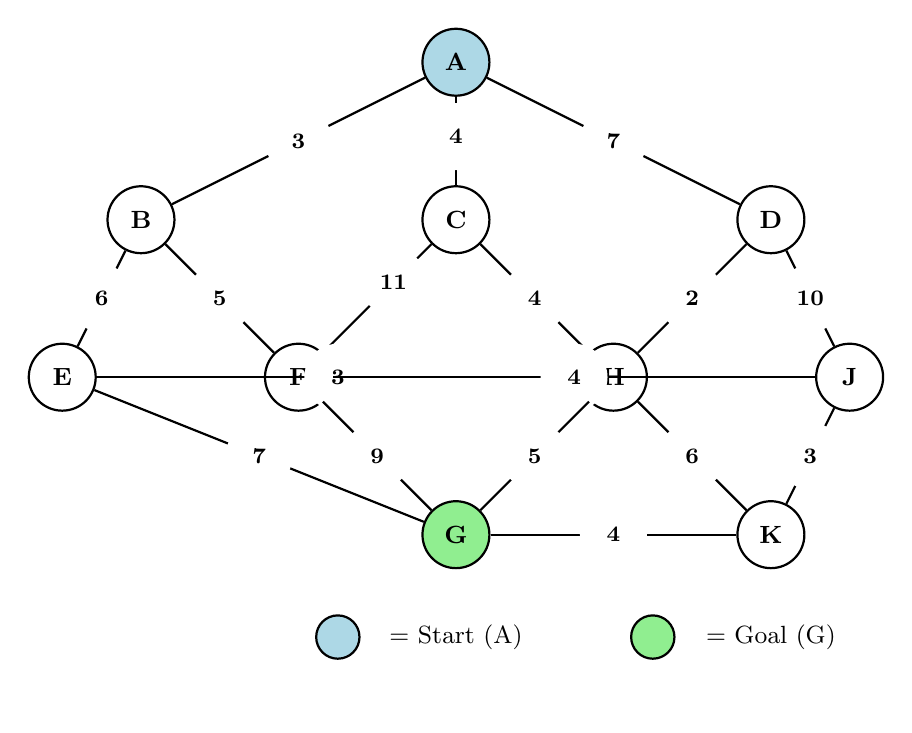
\begin{tikzpicture}[
  every node/.style={draw, circle, minimum size=0.85cm, inner sep=0pt,
                     font=\small\bfseries, thick},
  startnode/.style={fill=startblue},
  goalnode/.style={fill=goalgreen},
  lbl/.style={draw=none, fill=white, font=\footnotesize\bfseries,
               inner sep=1.5pt, outer sep=0pt},
  edge/.style={thick}
]

%--- Node positions ---
\node[startnode] (A) at (0, 6)   {A};
\node            (B) at (-4, 4)  {B};
\node            (C) at (0, 4)   {C};
\node            (D) at (4, 4)   {D};
\node            (E) at (-5, 2)  {E};
\node            (F) at (-2, 2)  {F};
\node            (H) at (2, 2)   {H};
\node            (J) at (5, 2)   {J};
\node            (K) at (4, 0)   {K};
\node[goalnode]  (G) at (0, 0)   {G};

%--- Edges ---
% Level A → B,C,D
\draw[edge] (A) -- node[lbl, pos=0.5] {3} (B);
\draw[edge] (A) -- node[lbl, pos=0.45] {4} (C);
\draw[edge] (A) -- node[lbl, pos=0.5] {7} (D);

% B → E, F
\draw[edge] (B) -- node[lbl, pos=0.5] {6} (E);
\draw[edge] (B) -- node[lbl, pos=0.5] {5} (F);

% C → F, H
\draw[edge] (C) -- node[lbl, pos=0.35] {11} (F);
\draw[edge] (C) -- node[lbl, pos=0.5]  {4}  (H);

% D → H, J
\draw[edge] (D) -- node[lbl, pos=0.5] {2}  (H);
\draw[edge] (D) -- node[lbl, pos=0.5] {10} (J);

% E → G   (diagonal, no crossing issue)
\draw[edge] (E) -- node[lbl, pos=0.5] {7} (G);

% E → H   (long horizontal — bent upward to avoid visual overlap with F)
\draw[edge, bend left=18] (E) -- node[lbl, pos=0.5] {3} (H);

% F → G
\draw[edge] (F) -- node[lbl, pos=0.5] {9} (G);

% F → J   (long horizontal — bent downward to clear node H)
\draw[edge, bend right=25] (F) -- node[lbl, pos=0.5] {4} (J);

% H → G, K
\draw[edge] (H) -- node[lbl, pos=0.5] {5} (G);
\draw[edge] (H) -- node[lbl, pos=0.5] {6} (K);

% J → K
\draw[edge] (J) -- node[lbl, pos=0.5] {3} (K);

% K → G
\draw[edge] (K) -- node[lbl, pos=0.5] {4} (G);

%--- Legend ---
\begin{scope}[shift={(0,-1.3)}]
  \node[startnode, minimum size=0.55cm, font=\tiny] (ls) at (-1.5,0) {};
  \node[draw=none, font=\small] at (0, 0) {= Start (A)};
  \node[goalnode, minimum size=0.55cm, font=\tiny] (lg) at (2.5,0)  {};
  \node[draw=none, font=\small] at (4, 0) {= Goal (G)};
\end{scope}

\end{tikzpicture}
\end{center}

\begin{notesbox}
\textbf{Note:} The edge E--H is curved upward and F--J is curved downward to avoid visual ambiguity where nodes share the same $y$-coordinate. All edges are \textbf{bidirectional} (undirected).
\end{notesbox}

%----------------------------------------------------------------------
\subsection{Part a(ii) — Search Algorithm Traces \ [5 marks]}
%----------------------------------------------------------------------

\begin{solutionbox}
\textbf{Question:} Show search trees for (1) UCS, (2) Greedy Best-First, (3) A*, (4) IDDFS from A to G.
At every step: show node being expanded and fringe contents in order of selection.
For IDDFS: show depth limit per iteration. Ties broken alphabetically.
\end{solutionbox}

\vspace{0.7em}

%----------------------------------------------------------------
\subsubsection*{Algorithm 1 — Uniform-Cost Search (UCS)}
%----------------------------------------------------------------

\textbf{Key idea:} Always expand the node with the \textbf{lowest path cost} $g(n)$ from the start.
The fringe is a \textbf{min-priority queue sorted by} $g(n)$.
A node is closed (never re-expanded) once popped.
If a \emph{cheaper} path to a fringe node is found, its cost is updated (replaced).

\textbf{Fringe notation:} Node$[g]$ sorted ascending by $g$.

\vspace{0.4em}
\begin{center}
\renewcommand{\arraystretch}{1.25}
\begin{tabular}{c|l|c|p{9.5cm}}
\toprule
\textbf{Step} & \textbf{Node Expanded} & \textbf{g(n)} &
\textbf{Fringe after expansion \ (sorted by g)} \\
\midrule
1 & \textbf{A} & 0
  & B[3], C[4], D[7] \\
  & & & \footnotesize Neighbours of A: B($g{=}3$), C($g{=}4$), D($g{=}7$). \\
\midrule
2 & \textbf{B} & 3
  & C[4], D[7], F[8], E[9] \\
  & & & \footnotesize A already closed. $B{\to}F$: $g{=}8$; $B{\to}E$: $g{=}9$. Both new.\\
\midrule
3 & \textbf{C} & 4
  & D[7], F[8], H[8], E[9] \\
  & & & \footnotesize $C{\to}F$: $g{=}15 > 8$ already in fringe $\Rightarrow$ keep $F[8]$. \
         $C{\to}H$: $g{=}8$ new. \\
\midrule
4 & \textbf{D} & 7
  & F[8], H[8], E[9], J[17] \\
  & & & \footnotesize $D{\to}H$: $g{=}9 > 8$ in fringe $\Rightarrow$ keep $H[8]$. \
         $D{\to}J$: $g{=}17$ new.
         Tie F,H: \textbf{F before H} (alphabetical). \\
\midrule
5 & \textbf{F} & 8
  & H[8], E[9], J[12], G[17] \\
  & & & \footnotesize $F{\to}G$: $g{=}17$ new. $F{\to}J$: $g{=}12 < 17$ in fringe
         $\Rightarrow$ \textbf{update} $J[12]$. \\
\midrule
6 & \textbf{H} & 8
  & E[9], J[12], G[13], K[14] \\
  & & & \footnotesize $H{\to}E$: $g{=}11 > 9$ in fringe $\Rightarrow$ keep $E[9]$. \
         $H{\to}G$: $g{=}13 < 17$ $\Rightarrow$ \textbf{update} $G[13]$. \
         $H{\to}K$: $g{=}14$ new. \\
\midrule
7 & \textbf{E} & 9
  & J[12], G[13], K[14] \\
  & & & \footnotesize $E{\to}G$: $g{=}16 > 13$ in fringe $\Rightarrow$ keep $G[13]$.\\
\midrule
8 & \textbf{J} & 12
  & G[13], K[14] \\
  & & & \footnotesize $J{\to}K$: $g{=}15 > 14$ in fringe $\Rightarrow$ keep $K[14]$.\\
\midrule
9 & \textbf{G} & 13
  & \goal \\
\bottomrule
\end{tabular}
\end{center}

\begin{answerbox}
\textbf{UCS Solution:} $A \;\xrightarrow{4}\; C \;\xrightarrow{4}\; H \;\xrightarrow{5}\; G$
\hfill \textbf{Total cost: $4+4+5 = \mathbf{13}$}

Nodes expanded (in order): A, B, C, D, F, H, E, J, G \quad(9 nodes total)

UCS \textbf{guarantees the optimal path} because it always expands the cheapest unexplored node, never re-expands a closed node, and path costs are non-negative.
\end{answerbox}

\vspace{1em}

%----------------------------------------------------------------
\subsubsection*{Algorithm 2 — Greedy Best-First Search}
%----------------------------------------------------------------

\textbf{Key idea:} Always expand the node with the \textbf{lowest heuristic estimate} $h(n)$ to the goal.
The fringe is sorted by $h(n)$ (ascending). Path cost $g(n)$ is \emph{completely ignored}.
Greedy is fast but not guaranteed to find the optimal path.

\textbf{Fringe notation:} Node$[h]$ sorted ascending by $h$.

\vspace{0.4em}
\begin{center}
\renewcommand{\arraystretch}{1.25}
\begin{tabular}{c|l|c|p{9cm}}
\toprule
\textbf{Step} & \textbf{Node Expanded} & \textbf{h(n)} &
\textbf{Fringe after expansion \ (sorted by h)} \\
\midrule
1 & \textbf{A} & 11
  & D[6], C[7], B[10] \\
  & & & \footnotesize Neighbours B($h{=}10$), C($h{=}7$), D($h{=}6$). Sorted by $h$: D, C, B. \\
\midrule
2 & \textbf{D} & 6
  & H[4], J[5], C[7], B[10] \\
  & & & \footnotesize D's neighbours excl.\ A: H($h{=}4$), J($h{=}5$). \\
\midrule
3 & \textbf{H} & 4
  & G[0], K[3], J[5], E[6], C[7], B[10] \\
  & & & \footnotesize H's neighbours excl.\ D: C($h{=}7$, already in fringe—skip),
         E($h{=}6$), G($h{=}0$), K($h{=}3$). \\
\midrule
4 & \textbf{G} & 0
  & \goal \\
\bottomrule
\end{tabular}
\end{center}

\begin{answerbox}
\textbf{Greedy Solution:} $A \;\xrightarrow{7}\; D \;\xrightarrow{2}\; H \;\xrightarrow{5}\; G$
\hfill \textbf{Total cost: $7+2+5 = \mathbf{14}$} (not optimal!)

Nodes expanded: A, D, H, G \quad(only 4 nodes — very fast)

Greedy expanded just 4 nodes versus UCS's 9, but found a \textbf{suboptimal path} (cost 14 vs optimal 13). It followed the heuristic blindly: D had the lowest $h$ from A, leading it down the D--H--G route instead of the cheaper A--C--H--G route.
\end{answerbox}

\vspace{1em}

%----------------------------------------------------------------
\subsubsection*{Algorithm 3 — A* Search}
%----------------------------------------------------------------

\textbf{Key idea:} Expand the node with the \textbf{lowest evaluation function}
$f(n) = g(n) + h(n)$, where $g(n)$ = exact cost from start and $h(n)$ = heuristic estimate to goal.
The fringe is sorted by $f(n)$ (ascending). Ties in $f$ broken alphabetically.
If a cheaper path to a fringe node is found, update its entry.

\textbf{Fringe notation:} Node$[g, h, f]$ sorted ascending by $f$.

\vspace{0.4em}
\begin{center}
\renewcommand{\arraystretch}{1.3}
\small
\begin{tabular}{c|l|c|c|c|p{7.2cm}}
\toprule
\textbf{Step} & \textbf{Node} & \textbf{g} & \textbf{h} & \textbf{f} &
\textbf{Fringe after expansion (sorted by f)} \\
\midrule
1 & \textbf{A} & 0 & 11 & 11
  & C[4,7,\textbf{11}], B[3,10,\textbf{13}], D[7,6,\textbf{13}] \\
  & & & & & \footnotesize Tie B,D at $f{=}13$: B first. \\
\midrule
2 & \textbf{C} & 4 & 7 & 11
  & H[8,4,\textbf{12}], B[3,10,\textbf{13}], D[7,6,\textbf{13}], F[15,6,\textbf{21}] \\
  & & & & & \footnotesize $C{\to}H$: $g{=}8,f{=}12$ new. $C{\to}F$: $g{=}15,f{=}21$ new. \\
\midrule
3 & \textbf{H} & 8 & 4 & 12
  & B[3,10,\textbf{13}], D[7,6,\textbf{13}], G[13,0,\textbf{13}], E[11,6,\textbf{17}], K[14,3,\textbf{17}], F[15,6,\textbf{21}] \\
  & & & & & \footnotesize $H{\to}D$: $f{=}16>13$, keep. $H{\to}G$: $f{=}13$ new. $H{\to}E$: $f{=}17$ new. $H{\to}K$: $f{=}17$ new. Tie B,D,G at $f{=}13$: \textbf{B first}. \\
\midrule
4 & \textbf{B} & 3 & 10 & 13
  & D[7,6,\textbf{13}], G[13,0,\textbf{13}], F[8,6,\textbf{14}], E[9,6,\textbf{15}], K[14,3,\textbf{17}] \\
  & & & & & \footnotesize $B{\to}F$: $g{=}8,f{=}14<21$ $\Rightarrow$ \textbf{update} F. $B{\to}E$: $g{=}9,f{=}15<17$ $\Rightarrow$ \textbf{update} E. Tie D,G at $f{=}13$: \textbf{D first}. \\
\midrule
5 & \textbf{D} & 7 & 6 & 13
  & G[13,0,\textbf{13}], F[8,6,\textbf{14}], E[9,6,\textbf{15}], K[14,3,\textbf{17}], J[17,5,\textbf{22}] \\
  & & & & & \footnotesize $D{\to}J$: $g{=}17,f{=}22$ new. \\
\midrule
6 & \textbf{G} & 13 & 0 & 13
  & \goal \\
\bottomrule
\end{tabular}
\end{center}

\begin{answerbox}
\textbf{A* Solution:} $A \;\xrightarrow{4}\; C \;\xrightarrow{4}\; H \;\xrightarrow{5}\; G$
\hfill \textbf{Total cost: $4+4+5 = \mathbf{13}$} (optimal!)

Nodes expanded: A, C, H, B, D, G \quad(6 nodes — fewer than UCS's 9)

A* is both \textbf{complete} and \textbf{optimal} when the heuristic is \emph{admissible} ($h(n) \leq h^*(n)$, i.e.\ it never overestimates). It is more efficient than UCS because $h(n)$ guides the search toward promising nodes, pruning unpromising directions early.
\end{answerbox}

\vspace{1em}

%----------------------------------------------------------------
\subsubsection*{Algorithm 4 — Iterative Deepening DFS (IDDFS)}
%----------------------------------------------------------------

\textbf{Key idea:} Perform DFS with a depth cutoff $L = 0, 1, 2, \ldots$, restarting from the root each time, until the goal is found. The ``fringe'' is a \textbf{stack} (LIFO). Children are pushed in \emph{reverse} alphabetical order so they are \emph{popped} (and expanded) in alphabetical order. Nodes on the \textbf{current path} (ancestors) are not revisited to avoid infinite loops.

\textbf{Stack notation:} Leftmost entry = top of stack (next to be popped). Depth shown in parentheses.

\vspace{0.5em}

\noindent\textbf{Iteration $L = 0$:}
\begin{center}
\renewcommand{\arraystretch}{1.2}
\begin{tabular}{c|l|p{8cm}}
\toprule
\textbf{Step} & \textbf{Action} & \textbf{Stack (top $\leftarrow$ left)} \\
\midrule
1 & Pop \textbf{A}(d=0). $A \neq G$. At depth limit — cannot expand. & $[\;\;]$ \\
\midrule
\multicolumn{3}{c}{\textit{No solution at $L=0$.}} \\
\bottomrule
\end{tabular}
\end{center}

\vspace{0.6em}

\noindent\textbf{Iteration $L = 1$:}
\begin{center}
\renewcommand{\arraystretch}{1.2}
\begin{tabular}{c|l|p{8cm}}
\toprule
\textbf{Step} & \textbf{Action} & \textbf{Stack} \\
\midrule
1 & Pop \textbf{A}(d=0). Expand: push D,C,B (B on top). & B(1), C(1), D(1) \\
2 & Pop \textbf{B}(d=1). $B \neq G$. At depth limit. & C(1), D(1) \\
3 & Pop \textbf{C}(d=1). $C \neq G$. At depth limit. & D(1) \\
4 & Pop \textbf{D}(d=1). $D \neq G$. At depth limit. & $[\;\;]$ \\
\midrule
\multicolumn{3}{c}{\textit{No solution at $L=1$.}} \\
\bottomrule
\end{tabular}
\end{center}

\vspace{0.6em}

\noindent\textbf{Iteration $L = 2$:}
\begin{center}
\renewcommand{\arraystretch}{1.2}
\begin{tabular}{c|l|p{8.5cm}}
\toprule
\textbf{Step} & \textbf{Action} & \textbf{Stack} \\
\midrule
1  & Pop \textbf{A}(d=0). Expand: B,C,D.
   & B(1), C(1), D(1) \\
2  & Pop \textbf{B}(d=1). Expand (excl.\ A): E,F. Push F,E.
   & E(2), F(2), C(1), D(1) \\
3  & Pop \textbf{E}(d=2). $E \neq G$. At limit.
   & F(2), C(1), D(1) \\
4  & Pop \textbf{F}(d=2). At limit.
   & C(1), D(1) \\
5  & Pop \textbf{C}(d=1). Expand (excl.\ A): F,H. Push H,F.
   & F(2), H(2), D(1) \\
6  & Pop \textbf{F}(d=2). At limit.
   & H(2), D(1) \\
7  & Pop \textbf{H}(d=2). At limit.
   & D(1) \\
8  & Pop \textbf{D}(d=1). Expand (excl.\ A): H,J. Push J,H.
   & H(2), J(2) \\
9  & Pop \textbf{H}(d=2). At limit.
   & J(2) \\
10 & Pop \textbf{J}(d=2). At limit.
   & $[\;\;]$ \\
\midrule
\multicolumn{3}{c}{\textit{No solution at $L=2$.}} \\
\bottomrule
\end{tabular}
\end{center}

\vspace{0.6em}

\noindent\textbf{Iteration $L = 3$:}
\begin{center}
\renewcommand{\arraystretch}{1.2}
\begin{tabular}{c|l|p{8.5cm}}
\toprule
\textbf{Step} & \textbf{Action} & \textbf{Stack} \\
\midrule
1 & Pop \textbf{A}(d=0). Expand: B,C,D.
  & B(1), C(1), D(1) \\
2 & Pop \textbf{B}(d=1). Expand (excl.\ A): E,F.
  & E(2), F(2), C(1), D(1) \\
3 & Pop \textbf{E}(d=2). Expand (excl.\ B): G,H. Push H first then G (G on top).
  & G(3), H(3), F(2), C(1), D(1) \\
4 & Pop \textbf{G}(d=3). $G = \mathrm{GOAL}$.
  & \goal \\
\bottomrule
\end{tabular}
\end{center}

\begin{answerbox}
\textbf{IDDFS Solution:} $A \;\xrightarrow{3}\; B \;\xrightarrow{6}\; E \;\xrightarrow{7}\; G$
\hfill \textbf{Depth: 3 \quad Cost: $3+6+7 = \mathbf{16}$}

IDDFS found the solution at depth-limit $L=3$ in just 4 node expansions during the final iteration.

\textbf{Important distinction:} IDDFS finds the \emph{shallowest} path (fewest hops), \textbf{not} the lowest-cost path. The optimal path A→C→H→G also has depth 3, but alphabetical DFS expansion reaches G via B→E→G first. For non-uniform step costs, IDDFS is \textbf{not optimal}. It is however \textbf{complete} — it will always find a solution if one exists.

\textbf{Why IDDFS over BFS?} IDDFS uses only $O(bL)$ \emph{space} (a single stack), whereas BFS requires $O(b^L)$ space to store all frontier nodes. The repeated work is a constant factor overhead.
\end{answerbox}

\vspace{0.8em}

\noindent\textbf{Algorithm Comparison Summary:}
\begin{center}
\renewcommand{\arraystretch}{1.3}
\begin{tabular}{l|l|c|c|c}
\toprule
\textbf{Algorithm} & \textbf{Path Found} & \textbf{Cost} & \textbf{Nodes Expanded} & \textbf{Optimal?} \\
\midrule
UCS    & A → C → H → G & 13 & 9 (all iterations) & \textbf{Yes} \\
Greedy & A → D → H → G & 14 & 4                  & No \\
A*     & A → C → H → G & 13 & 6                  & \textbf{Yes} \\
IDDFS  & A → B → E → G & 16 & 4 (final iter.)    & No (non-uniform costs) \\
\bottomrule
\end{tabular}
\end{center}

%----------------------------------------------------------------------
\subsection{Part b — Problem Formulations \ [3 marks]}
%----------------------------------------------------------------------

\begin{solutionbox}
\textbf{Question:} Give the initial state, goal test, operators, and path cost function for each problem.
\end{solutionbox}

\subsubsection*{(i) Robot Vacuum Cleaning Problem (Indoor Environment)}

\begin{description}[leftmargin=3.2cm, labelwidth=3cm, labelsep=0.2cm]
  \item[\textbf{State:}]
    A pair $(\,l,\; D\,)$ where $l$ is the robot's current room and $D \subseteq \{\text{all rooms}\}$ is the set of dirty rooms.
    \emph{Example:} $(\text{Kitchen},\; \{\text{Bedroom, Lounge}\})$.

  \item[\textbf{Initial state:}]
    $(\text{start room},\; \{\text{all currently dirty rooms}\})$.

  \item[\textbf{Goal test:}]
    $D = \emptyset$ \quad (no dirty rooms remain).

  \item[\textbf{Operators:}]
    \begin{enumerate}[noitemsep]
      \item $\mathrm{Move}(r_i \to r_j)$: Move from room $r_i$ to adjacent room $r_j$ (changes location; $D$ unchanged).
      \item $\mathrm{Suck}()$: Vacuum the current room (removes current room from $D$ if dirty).
    \end{enumerate}
    Static obstacles (furniture) constrain which rooms are adjacent.

  \item[\textbf{Path cost:}]
    Total energy used: each $\mathrm{Move}$ costs $c_{\mathrm{move}}$ energy units; each $\mathrm{Suck}$ costs $c_{\mathrm{suck}}$ units. Goal: minimise total energy.

  \item[\textbf{Informed vs.\ Uninformed:}]
    \textbf{Informed search (A*) is more suitable.} A strong heuristic $h(n) = |D| \times \overline{d}$ (number of remaining dirty rooms multiplied by average travel cost between rooms) estimates remaining work without overestimating. With many rooms, uninformed BFS/UCS must explore exponentially many $(l, D)$ state combinations blindly. A* with a good heuristic dramatically prunes this search space.
\end{description}

\subsubsection*{(ii) Water Jug Problem (5L and 3L Jugs)}

\begin{description}[leftmargin=3.2cm, labelwidth=3cm, labelsep=0.2cm]
  \item[\textbf{State:}]
    A pair $(\,x,\; y\,)$ where $x \in \{0,1,2,3,4,5\}$ is water (litres) in the 5L jug and $y \in \{0,1,2,3\}$ is water in the 3L jug.

  \item[\textbf{Initial state:}]
    $(0,\; 0)$ — both jugs empty.

  \item[\textbf{Goal test:}]
    $x = 4$ (exactly 4 litres in the 5L jug). The 3L jug cannot hold 4L, so only $x=4$ satisfies the goal.

  \item[\textbf{Operators:}]
    \begin{enumerate}[noitemsep]
      \item \textbf{Fill 5L:} $(x,y) \to (5,\;y)$
      \item \textbf{Fill 3L:} $(x,y) \to (x,\;3)$
      \item \textbf{Empty 5L:} $(x,y) \to (0,\;y)$
      \item \textbf{Empty 3L:} $(x,y) \to (x,\;0)$
      \item \textbf{Pour 5L $\to$ 3L:} $(x,y) \to (x{-}d,\;y{+}d)$ where $d = \min(x,\; 3{-}y)$
      \item \textbf{Pour 3L $\to$ 5L:} $(x,y) \to (x{+}d,\;y{-}d)$ where $d = \min(y,\; 5{-}x)$
    \end{enumerate}

  \item[\textbf{Path cost:}]
    Number of actions performed (1 per action), minimised to find the shortest sequence.

  \item[\textbf{State space:}]
    \textbf{FINITE.} The 5L jug holds integer amounts $\{0,1,2,3,4,5\}$ (6 values) and the 3L jug holds $\{0,1,2,3\}$ (4 values), giving at most $6 \times 4 = 24$ states. Not all are reachable, but the space is strictly bounded.

    \textit{One valid solution path (6 steps):}
    \[
    (0,0)
    \xrightarrow{\mathrm{Fill\,5L}} (5,0)
    \xrightarrow{\mathrm{Pour\,5\to3}} (2,3)
    \xrightarrow{\mathrm{Empty\,3L}} (2,0)
    \xrightarrow{\mathrm{Pour\,5\to3}} (0,2)
    \xrightarrow{\mathrm{Fill\,5L}} (5,2)
    \xrightarrow{\mathrm{Pour\,5\to3}} (4,3)
    \quad \Rightarrow x=4 \;\checkmark
    \]
\end{description}

%=====================================================================
\newpage
\section{Examination 2023 — Q2 \ (9 Marks)}
%=====================================================================

\subsection{Problem Data}

\begin{minipage}[t]{0.46\textwidth}
\centering
{\small\textbf{Table 1: State Transitions and Step Costs}}\\[0.4em]
\begin{tabular}{ccc}
\toprule
\textbf{State} & \textbf{Next} & \textbf{Cost} \\
\midrule
A & B & 4 \\
A & C & 1 \\
B & D & 3 \\
B & E & 8 \\
C & C & 0 \\
C & D & 2 \\
C & F & 6 \\
D & C & 2 \\
D & E & 4 \\
E & G & 2 \\
F & G & 8 \\
\bottomrule
\end{tabular}
\end{minipage}
\hfill
\begin{minipage}[t]{0.46\textwidth}
\centering
{\small\textbf{Table 2: Heuristic Estimates $h(n)$}}\\[0.4em]
\begin{tabular}{cc}
\toprule
\textbf{Node} & \textbf{h(n)} \\
\midrule
A & 8 \\
B & 8 \\
C & 6 \\
D & 5 \\
E & 1 \\
F & 4 \\
G & 0 \\
\bottomrule
\end{tabular}
\end{minipage}

\vspace{0.6em}
\begin{notesbox}
\textbf{Important:} This is a \textbf{directed} graph — edges go one way only (State $\to$ Next). Note the self-loop C$\to$C with cost 0 — this is a degenerate edge and should be ignored during search (it does not change the state or advance toward the goal). Also note the edge D$\to$C(2): returning from D to C is allowed since the graph is directed — C is reachable from both A and D. No reverse edges from B$\to$A, C$\to$A, D$\to$B, etc.\ exist unless listed in the table above.
\end{notesbox}

%----------------------------------------------------------------------
\subsection{Part a — Problem Formulations \ [2 marks]}
%----------------------------------------------------------------------

\begin{solutionbox}
\textbf{Question:} Give the initial state, goal test, operators, and path cost for each problem.
\end{solutionbox}

\subsubsection*{(i) Travelling Salesman Problem (TSP)}

\begin{description}[leftmargin=3.6cm, labelwidth=3.4cm, labelsep=0.2cm]
  \item[\textbf{State:}]
    A pair $(\,\ell,\; V\,)$ where $\ell$ is the current city and $V \subseteq \{\text{all } N \text{ cities}\}$ is the set of \emph{unvisited} cities.
    \emph{Example midway:} $(\text{Dhaka},\; \{\text{Chittagong, Sylhet}\})$ means we are in Dhaka and still need to visit Chittagong and Sylhet.

  \item[\textbf{Initial state:}]
    $(\text{start city},\; \{\text{all } N{-}1 \text{ other cities}\})$.

  \item[\textbf{Goal test:}]
    $\ell = \text{start city}$ \textbf{and} $V = \emptyset$ \quad (returned to start after visiting all cities exactly once).

  \item[\textbf{Operators:}]
    $\text{Travel}(\text{city}_i \to \text{city}_j)$ where city$_j \notin V$ or ($V{=}\emptyset$ and city$_j{=}$start). Each move removes city$_j$ from $V$.

  \item[\textbf{Path cost:}]
    Sum of distances (or costs) of all travelled roads. Goal: find the tour with \textbf{minimum total cost}.

  \item[\textbf{Complexity note:}]
    With $N$ cities there are $(N{-}1)!/2$ distinct tours — factorial growth. TSP is NP-hard, so exhaustive search is infeasible for $N>20$. Heuristic search (A*) with an admissible heuristic (e.g.\ minimum spanning tree of remaining cities) can find optimal or near-optimal tours for moderate $N$.
\end{description}

\subsubsection*{(ii) Missionaries \& Cannibals}

\begin{description}[leftmargin=3.6cm, labelwidth=3.4cm, labelsep=0.2cm]
  \item[\textbf{State:}]
    A triple $(\,M_L,\; C_L,\; B\,)$ where $M_L$ = missionaries on left bank ($0$–$3$), $C_L$ = cannibals on left bank ($0$–$3$), $B \in \{L,R\}$ = boat position.
    The right bank has $3{-}M_L$ missionaries and $3{-}C_L$ cannibals.

  \item[\textbf{Initial state:}]
    $(3,\; 3,\; L)$ — all six people and the boat on the left bank.

  \item[\textbf{Goal test:}]
    $(0,\; 0,\; R)$ — all six people and the boat on the right bank.

  \item[\textbf{Operators:}]
    Move $k$ missionaries and $j$ cannibals across the river \textbf{by boat}, where $1 \leq k{+}j \leq 2$ (boat capacity 2), and the resulting state must be \textbf{legal}: on both banks, $M \geq C$ \emph{or} $M=0$ (missionaries never outnumbered by cannibals on either side).

    \emph{Possible boat loads:} (1M,0C), (2M,0C), (0M,1C), (0M,2C), (1M,1C).

  \item[\textbf{Path cost:}]
    Number of boat trips (1 per crossing). Goal: find a sequence with \textbf{minimum trips}.

  \item[\textbf{State space size:}]
    Without constraints: $4 \times 4 \times 2 = 32$ states. After legality filtering, only about 16–20 are valid. The problem has a known shortest solution of \textbf{11 crossings}.
\end{description}

%----------------------------------------------------------------------
\subsection{Part b(i) — State-Space Diagram \ [0.5 mark]}
%----------------------------------------------------------------------

\begin{center}
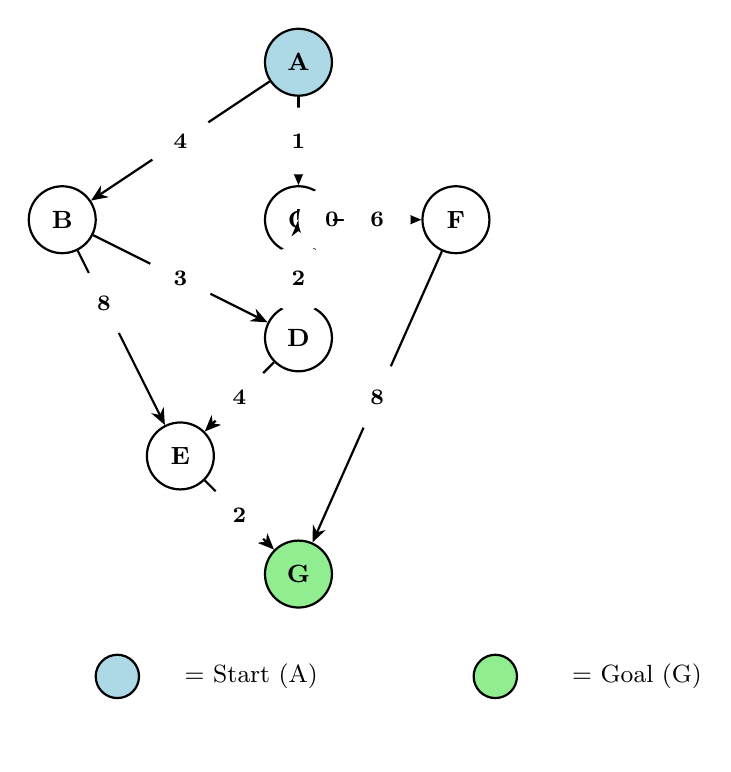
\begin{tikzpicture}[
  every node/.style={draw, circle, minimum size=0.85cm, inner sep=0pt,
                     font=\small\bfseries, thick},
  startnode/.style={fill=startblue},
  goalnode/.style={fill=goalgreen},
  lbl/.style={draw=none, fill=white, font=\footnotesize\bfseries,
               inner sep=1.5pt, outer sep=0pt},
  edge/.style={thick, -{Stealth[length=6pt, width=5pt]}}
]

%--- Node positions ---
\node[startnode] (A) at (0, 5)   {A};
\node            (B) at (-3, 3)  {B};
\node            (C) at (0, 3)   {C};
\node            (D) at (0, 1.5) {D};
\node            (E) at (-1.5, 0) {E};
\node            (F) at (2, 3)   {F};
\node[goalnode]  (G) at (0, -1.5) {G};

%--- Directed edges ---
\draw[edge]              (A) -- node[lbl, pos=0.5] {4} (B);
\draw[edge, bend left=10] (A) -- node[lbl, pos=0.5] {1} (C);
\draw[edge]              (B) -- node[lbl, pos=0.5] {3} (D);
\draw[edge, bend right=20] (B) -- node[lbl, pos=0.3] {8} (E);
\draw[edge, loop right]  (C) -- node[lbl, pos=0.5] {0} (C);
\draw[edge]              (C) -- node[lbl, pos=0.5] {2} (D);
\draw[edge, bend left=20] (C) -- node[lbl, pos=0.5] {6} (F);
\draw[edge, bend right=15] (D) -- node[lbl, pos=0.5] {2} (C);
\draw[edge]              (D) -- node[lbl, pos=0.5] {4} (E);
\draw[edge]              (E) -- node[lbl, pos=0.5] {2} (G);
\draw[edge]              (F) -- node[lbl, pos=0.5] {8} (G);

%--- Legend ---
\begin{scope}[shift={(-0.5,-2.8)}]
  \node[startnode, minimum size=0.55cm, font=\tiny] (ls) at (-1.8,0) {};
  \node[draw=none, font=\small] at (-0.1, 0) {= Start (A)};
  \node[goalnode, minimum size=0.55cm, font=\tiny] (lg) at (3,0)  {};
  \node[draw=none, font=\small] at (4.8, 0) {= Goal (G)};
\end{scope}

\end{tikzpicture}
\end{center}

\begin{notesbox}
\textbf{Notes on the graph structure:}
\begin{itemize}[noitemsep,topsep=2pt]
  \item C$\to$C(0) is a zero-cost self-loop — degenerate; ignored in search.
  \item D$\to$C(2) creates a directed 2-cycle C $\rightleftharpoons$ D (C$\to$D costs 2, D$\to$C costs 2).
  \item B has two outgoing edges: B$\to$D(3) and B$\to$E(8). B$\to$E is an expensive direct path.
  \item The cheap route to the goal passes through D$\to$E(4)$\to$G(2).
  \item From A, the best first step is C (cost 1), not B (cost 4).
\end{itemize}
\end{notesbox}

%----------------------------------------------------------------------
\subsection{Part b(ii) — Search Algorithm Traces \ [4.5 marks]}
%----------------------------------------------------------------------

\begin{solutionbox}
\textbf{Question:} Trace UCS, Greedy search, and A* from A (initial) to G (goal).
At each step: show the node being expanded and the fringe contents.
Ties broken alphabetically.
\end{solutionbox}

\vspace{0.7em}

%----------------------------------------------------------------
\subsubsection*{Algorithm 1 — Uniform-Cost Search (UCS)}
%----------------------------------------------------------------

\textbf{Key idea:} Expand the node with the \textbf{lowest path cost} $g(n)$. Fringe is a min-priority queue sorted by $g(n)$.
Once a node is expanded (closed), it is never re-expanded. If a cheaper path to a fringe node is found, update its cost.

\textbf{Fringe notation:} Node$[g]$ sorted ascending by $g$.
\textbf{Closed set:} $\{\text{nodes already expanded}\}$.

\vspace{0.4em}
\begin{center}
\renewcommand{\arraystretch}{1.3}
\small
\begin{tabular}{c|l|c|p{9cm}}
\toprule
\textbf{Step} & \textbf{Node} & \textbf{g} &
\textbf{Fringe after expansion \ (sorted by g)} \\
\midrule
1 & \textbf{A} & 0
  & C[\textbf{1}],\; B[\textbf{4}] \\
  & & & \footnotesize $A{\to}C$: $g{=}1$. $A{\to}B$: $g{=}4$. Both new. \\
\midrule
2 & \textbf{C} & 1
  & D[\textbf{3}],\; B[\textbf{4}],\; F[\textbf{7}] \\
  & & & \footnotesize $C{\to}C$: self-loop, ignore. $C{\to}D$: $g{=}3$ new. $C{\to}F$: $g{=}7$ new. \\
\midrule
3 & \textbf{D} & 3
  & B[\textbf{4}],\; E[\textbf{7}],\; F[\textbf{7}] \\
  & & & \footnotesize $D{\to}C$: $g{=}5$, C already closed $\Rightarrow$ skip. $D{\to}E$: $g{=}7$ new. \\
\midrule
4 & \textbf{B} & 4
  & E[\textbf{7}],\; F[\textbf{7}] \\
  & & & \footnotesize $B{\to}D$: $g{=}7$, D already closed $\Rightarrow$ skip. $B{\to}E$: $g{=}12 > \text{E[7]}$ in fringe $\Rightarrow$ keep E[7]. \\
\midrule
5 & \textbf{E} & 7
  & F[\textbf{7}],\; G[\textbf{9}] \\
  & & & \footnotesize Tie E[7], F[7]: \textbf{E before F} (alphabetical). $E{\to}G$: $g{=}9$ new. \\
\midrule
6 & \textbf{F} & 7
  & G[\textbf{9}] \\
  & & & \footnotesize $F{\to}G$: $g{=}15 > \text{G[9]}$ in fringe $\Rightarrow$ keep G[9]. \\
\midrule
7 & \textbf{G} & 9
  & \goal \\
\bottomrule
\end{tabular}
\end{center}

\begin{answerbox}
\textbf{UCS Solution:} $A \;\xrightarrow{1}\; C \;\xrightarrow{2}\; D \;\xrightarrow{4}\; E \;\xrightarrow{2}\; G$
\hfill \textbf{Total cost: $1+2+4+2 = \mathbf{9}$}

Nodes expanded (in order): A, C, D, B, E, F, G \quad(7 nodes total)

UCS guarantees the optimal path because it explores in order of increasing $g(n)$ and step costs are non-negative.
\end{answerbox}

\vspace{1em}

%----------------------------------------------------------------
\subsubsection*{Algorithm 2 — Greedy Best-First Search}
%----------------------------------------------------------------

\textbf{Key idea:} Expand the node with the \textbf{lowest heuristic} $h(n)$. Fringe sorted by $h$ ascending.
Path cost $g(n)$ is \emph{completely ignored}. This is fast but not guaranteed optimal.

\textbf{Fringe notation:} Node$[h]$ sorted ascending by $h$.

\vspace{0.4em}
\begin{center}
\renewcommand{\arraystretch}{1.3}
\small
\begin{tabular}{c|l|c|p{9cm}}
\toprule
\textbf{Step} & \textbf{Node} & \textbf{h} &
\textbf{Fringe after expansion \ (sorted by h)} \\
\midrule
1 & \textbf{A} & 8
  & C[\textbf{6}],\; B[\textbf{8}] \\
  & & & \footnotesize $A{\to}C$: $h{=}6$. $A{\to}B$: $h{=}8$. \\
\midrule
2 & \textbf{C} & 6
  & F[\textbf{4}],\; D[\textbf{5}],\; B[\textbf{8}] \\
  & & & \footnotesize $C{\to}F$: $h{=}4$. $C{\to}D$: $h{=}5$. $C{\to}C$ ignored. \\
\midrule
3 & \textbf{F} & 4
  & G[\textbf{0}],\; D[\textbf{5}],\; B[\textbf{8}] \\
  & & & \footnotesize $F{\to}G$: $h{=}0$. Goal in fringe with lowest $h$. \\
\midrule
4 & \textbf{G} & 0
  & \goal \\
\bottomrule
\end{tabular}
\end{center}

\begin{answerbox}
\textbf{Greedy Solution:} $A \;\xrightarrow{1}\; C \;\xrightarrow{6}\; F \;\xrightarrow{8}\; G$
\hfill \textbf{Total cost: $1+6+8 = \mathbf{15}$} (suboptimal!)

Nodes expanded: A, C, F, G \quad(only 4 nodes — extremely fast)

Greedy blindly chased the heuristic: from C, F has $h{=}4$ (lowest), so it went C$\to$F, but F$\to$G costs 8 — the most expensive path to the goal. It completely missed the cheap C$\to$D$\to$E$\to$G route (cost 9) because D's $h{=}5$ looked slightly worse than F's $h{=}4$.
\end{answerbox}

\vspace{1em}

%----------------------------------------------------------------
\subsubsection*{Algorithm 3 — A* Search}
%----------------------------------------------------------------

\textbf{Key idea:} Expand the node with the \textbf{lowest $f(n) = g(n) + h(n)$}. Fringe sorted by $f$ ascending.
Ties in $f$ broken alphabetically. Closed set prevents re-expansion.

\textbf{Fringe notation:} Node$[g,\; h,\; f]$ sorted ascending by $f$.

\vspace{0.4em}
\begin{center}
\renewcommand{\arraystretch}{1.35}
\scriptsize
\begin{tabular}{c|l|c|c|c|p{7.5cm}}
\toprule
\textbf{Step} & \textbf{Node} & \textbf{g} & \textbf{h} & \textbf{f} &
\textbf{Fringe after expansion (sorted by f)} \\
\midrule
1 & \textbf{A} & 0 & 8 & 8
  & C[1,6,\textbf{7}],\; B[4,8,\textbf{12}] \\
  & & & & & \footnotesize $A{\to}C$: $f{=}1{+}6{=}7$. $A{\to}B$: $f{=}4{+}8{=}12$. \\
\midrule
2 & \textbf{C} & 1 & 6 & 7
  & D[3,5,\textbf{8}],\; F[7,4,\textbf{11}],\; B[4,8,\textbf{12}] \\
  & & & & & \footnotesize $C{\to}D$: $g{=}3,f{=}8$. $C{\to}F$: $g{=}7,f{=}11$. C$\to$C ignored. \\
\midrule
3 & \textbf{D} & 3 & 5 & 8
  & E[7,1,\textbf{8}],\; F[7,4,\textbf{11}],\; B[4,8,\textbf{12}] \\
  & & & & & \footnotesize $D{\to}C$: C closed $\Rightarrow$ skip. $D{\to}E$: $g{=}7,f{=}8$. \\
  & & & & & \footnotesize Tie D($f{=}8$) and E($f{=}8$): D already expanded, E is in fringe. \\
\midrule
4 & \textbf{E} & 7 & 1 & 8
  & G[9,0,\textbf{9}],\; F[7,4,\textbf{11}],\; B[4,8,\textbf{12}] \\
  & & & & & \footnotesize $E{\to}G$: $g{=}9,f{=}9$. \\
\midrule
5 & \textbf{G} & 9 & 0 & 9
  & \goal \\
\bottomrule
\end{tabular}
\end{center}

\begin{answerbox}
\textbf{A* Solution:} $A \;\xrightarrow{1}\; C \;\xrightarrow{2}\; D \;\xrightarrow{4}\; E \;\xrightarrow{2}\; G$
\hfill \textbf{Total cost: $1+2+4+2 = \mathbf{9}$} (optimal!)

Nodes expanded: A, C, D, E, G \quad(only 5 nodes — fewer than UCS's 7)

A* found the optimal path and expanded \textbf{only 5 nodes} compared to UCS's 7, because the heuristic $h(n)$ guided it away from the expensive B and F branches. Note that \textbf{B was never expanded} — its $f{=}12$ was always worse than the alternatives ahead of it in the fringe.
\end{answerbox}

\vspace{0.8em}

\noindent\textbf{Algorithm Comparison for 2023 Graph:}
\begin{center}
\renewcommand{\arraystretch}{1.3}
\begin{tabular}{l|l|c|c|c}
\toprule
\textbf{Algorithm} & \textbf{Path Found} & \textbf{Cost} & \textbf{Nodes Expanded} & \textbf{Optimal?} \\
\midrule
UCS    & A $\to$ C $\to$ D $\to$ E $\to$ G & \textbf{9} & 7 & \textbf{Yes} \\
Greedy & A $\to$ C $\to$ F $\to$ G          & 15 & 4 & No \\
A*     & A $\to$ C $\to$ D $\to$ E $\to$ G & \textbf{9} & 5 & \textbf{Yes} \\
\bottomrule
\end{tabular}
\end{center}

\begin{notesbox}
\textbf{Why does A* outperform UCS here?} The heuristic $h(n)$ provides a useful lower bound. After expanding A and C, A* sees that D has $f{=}8$ (promising — $h(D){=}5$ is close to the true remaining cost of 6) while B has $f{=}12$ (unpromising — $h(B){=}8$ overestimates its potential). A* expands D next and finds the optimal path without ever touching B. UCS, lacking a heuristic, expands B unnecessarily at step 4 before reaching the goal.

\textbf{Admissibility check:} Is $h(n)$ admissible? Let's verify:
\begin{itemize}[noitemsep,topsep=3pt]
  \item $h(A){=}8 \leq h^*(A){=}9$ \checkmark
  \item $h(C){=}6 \leq h^*(C){=}8$ \checkmark
  \item $h(D){=}5 \leq h^*(D){=}6$ \checkmark
  \item $h(E){=}1 \leq h^*(E){=}2$ \checkmark
  \item $h(B){=}8 \leq h^*(B){=}5$? \textbf{No!} $h^*(B) = \min(3{+}4{+}2,\; 8{+}2) = 9$. Wait — $B{\to}D{\to}E{\to}G = 3{+}4{+}2=9$, so $h(B){=}8 < 9$ \checkmark. And $B{\to}E{\to}G = 8{+}2=10$. So $h^*(B){=}9$, $h(B){=}8$ is admissible.
  \item $h(F){=}4 \leq h^*(F){=}8$ \checkmark
\end{itemize}
\textbf{Yes, the heuristic is admissible} — $h(n) \leq h^*(n)$ for all nodes. This is why A* found the optimal solution.
\end{notesbox}

%----------------------------------------------------------------------
\subsection{Part c — IDDFS: Synthesising Benefits of BFS and DFS \ [2 marks]}
%----------------------------------------------------------------------

\begin{solutionbox}
\textbf{Question:} Illustrate with an appropriate example how IDDFS synthesises the benefits of both BFS and DFS — achieving optimality, completeness, and linear space complexity. Nevertheless, time complexity deteriorates in comparison to both BFS and DFS.
\end{solutionbox}

\vspace{0.6em}

\subsubsection*{The Core Idea}

IDDFS (Iterative Deepening Depth-First Search) runs DFS repeatedly with an increasing depth cutoff: first $L{=}0$, then $L{=}1$, $L{=}2$, \ldots, until the goal is found. At each iteration, the search is a standard depth-limited DFS from the root.

\subsubsection*{Illustrative Example}

Consider the following binary tree where G (shaded) is the shallowest goal at depth 3:

\begin{center}
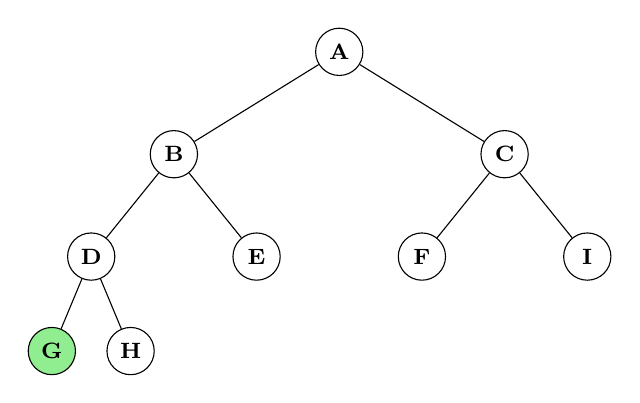
\begin{tikzpicture}[
  level 1/.style={sibling distance=4.2cm, level distance=1.3cm},
  level 2/.style={sibling distance=2.1cm, level distance=1.3cm},
  level 3/.style={sibling distance=1.0cm, level distance=1.2cm},
  every node/.style={draw, circle, minimum size=0.6cm, inner sep=0pt, font=\footnotesize\bfseries},
  goalnode/.style={fill=goalgreen},
  edgelbl/.style={draw=none, font=\footnotesize, inner sep=1pt}
]
\node {A}
  child { node {B}
    child { node {D}
      child { node[goalnode] {G} }
      child { node {H} }
    }
    child { node {E} }
  }
  child { node {C}
    child { node {F} }
    child { node {I} }
  };
\end{tikzpicture}
\end{center}

\vspace{0.4em}

\noindent\textbf{IDDFS Execution:}

\begin{center}
\renewcommand{\arraystretch}{1.2}
\small
\begin{tabular}{c|l|p{9cm}}
\toprule
\textbf{L} & \textbf{Nodes visited (DFS order)} & \textbf{Outcome} \\
\midrule
0 & A & A $\neq$ G. No solution at depth 0. \\
1 & A, B, C & Neither B nor C is G. No solution at depth 1. \\
2 & A, B, D, E, C, F, I & No goal at depth 2. \\
3 & A, B, D, \textbf{G} $\leftarrow$ \goal & \textbf{Found!} Shallowest goal at depth 3. \\
\bottomrule
\end{tabular}
\end{center}

\subsubsection*{How IDDFS Inherits Each Algorithm's Strengths}

\begin{center}
\renewcommand{\arraystretch}{1.4}
\begin{tabular}{l|p{5cm}|p{5cm}|p{5cm}}
\toprule
\textbf{Property} & \textbf{BFS} & \textbf{DFS} & \textbf{IDDFS} \\
\midrule
\textbf{Completeness} &
  \checkmark\ Complete (finds solution if one exists) &
  \texttimes\ Incomplete (may loop forever on infinite branches) &
  \checkmark\ \textbf{Complete} — like BFS. Depth-limited DFS avoids infinite loops because it backtracks at the cutoff. \\
\midrule
\textbf{Optimality} &
  \checkmark\ Optimal for uniform step costs (finds shallowest solution) &
  \texttimes\ Not optimal (may find a deep solution first) &
  \checkmark\ \textbf{Optimal for uniform costs} — like BFS. Because it explores all nodes at depth $d{-}1$ before any at depth $d$, the first solution found is the shallowest. \\
\midrule
\textbf{Space} &
  \texttimes\ $O(b^d)$ — stores entire frontier. For $b{=}10,d{=}10$, that's 10 billion nodes. &
  \checkmark\ $O(bm)$ — stores only one path + siblings. &
  \checkmark\ \textbf{$O(bd)$} — like DFS. Only the current path (depth $d$) plus $b{-}1$ siblings per level are in memory. For $b{=}10,d{=}10$: $\approx$ 100 nodes. \\
\midrule
\textbf{Time} &
  $O(b^d)$ — visits each node once &
  $O(b^m)$ — may go very deep, but each node visited once &
  \texttimes\ $O(b^d)$ — \textbf{worse constant factor.} Nodes near the root are revisited $d$ times. Overhead factor: $\frac{b}{b-1}$ (e.g.\ for $b{=}10$, about $1.11\times$ BFS). \\
\bottomrule
\end{tabular}
\end{center}

\subsubsection*{Why Time Complexity Deteriorates}

The key weakness of IDDFS is \textbf{repeated work}. Consider the root node A: it is expanded in \emph{every} iteration ($L{=}0,1,2,3$) — 4 times. Node B is expanded at $L{=}2$ and $L{=}3$ — twice. Only the deepest nodes (depth $L$) are expanded just once.

However, in a tree with branching factor $b$, the \textbf{number of nodes at the deepest level dominates}:
\[
\text{Total expansions} = (d{+}1) \cdot 1 + d \cdot b + (d{-}1) \cdot b^2 + \cdots + 1 \cdot b^d
\]
\[
= b^d \left(1 + \frac{1}{b} + \frac{1}{b^2} + \cdots\right)
\approx b^d \cdot \frac{b}{b-1}
\]

For $b=10$, the overhead is only $\frac{10}{9} \approx 1.11\times$ — a small price for the enormous space savings ($O(bd)$ vs $O(b^d)$). This is why IDDFS is the \textbf{preferred uninformed search strategy} when the state space is large and step costs are uniform.

\subsubsection*{When IDDFS Is NOT Optimal}

IDDFS finds the \textbf{shallowest} goal (fewest edges), not the lowest-cost goal. With non-uniform step costs, a deeper path with lower total cost may exist. In such cases, UCS or A* is required. For the 2024 exam graph, IDDFS found A$\to$B$\to$E$\to$G (cost 16, 3 hops) while UCS found A$\to$C$\to$H$\to$G (cost 13, 3 hops) — both at the same depth, but UCS found the cheaper one because it considers edge costs, not just depth.

\begin{notesbox}
\textbf{Exam summary — IDDFS:}
\begin{itemize}[noitemsep,topsep=2pt]
  \item \textbf{Completeness:} Inherited from BFS — guaranteed to find a solution if one exists.
  \item \textbf{Optimality:} Inherited from BFS — optimal for \emph{uniform} step costs (finds shallowest solution).
  \item \textbf{Space:} Inherited from DFS — $O(bd)$ linear space, practical for large search spaces.
  \item \textbf{Time:} Worse than both BFS and DFS individually — nodes near the root are re-expanded each iteration. However, the overhead is only a constant factor ($\approx \frac{b}{b-1}$), acceptable given the space savings.
\end{itemize}
\end{notesbox}

\end{document}
